% This is samplepaper.tex, a sample chapter demonstrating the
% LLNCS macro package for Springer Computer Science proceedings;
% Version 2.20 of 2017/10/04
%
\documentclass[runningheads]{llncs}
%
\usepackage{graphicx}
\usepackage{color}
\usepackage{amsmath,amssymb}
\usepackage{multicol}
\usepackage[misc]{ifsym}
\usepackage{times}

% Used for displaying a sample figure. If possible, figure files should
% be included in EPS format.
%
% If you use the hyperref package, please uncomment the following line
% to display URLs in blue roman font according to Springer's eBook style:
% \renewcommand\UrlFont{\color{blue}\rmfamily}



%\usepackage{microtype}
 \newcommand{\myspace}{\vspace*{-0.5em}}
 \newcommand{\mybigspace}{\vspace*{-1em}}
 \renewcommand{\baselinestretch}{1} % >=0.97
% \advance\textwidth5mm % <= 5mm
% \advance\hoffset-3mm
% \advance\textheight6mm
% \advance\voffset-3mm
 
 % == TITLESEC ==
 
 % Save the class definition of \subparagraph
 \let\llncssubparagraph\subparagraph
 % Provide a definition to \subparagraph to keep titlesec happy
 \let\subparagraph\paragraph
 % Load titlesec
 \usepackage[compact]{titlesec}
 % Revert \subparagraph to the llncs definition
 \let\subparagraph\llncssubparagraph
 
 \titlespacing*{\section}{0pt}{0.7em plus 0.2em minus 0.1em}{0.4em plus 0.05em}
 \titlespacing*{\subsection}{0pt}{0.5em plus 0.1em minus 0.1em}{0.3em plus 0.05em}



\begin{document}
%
\title{Approximating Complex Arithmetic Circuits with Guaranteed Worst-Case
Relative Error\thanks{This work has been partially supported by the Brno Ph.D.
Scholarship Program, the Czech Science Foundation (project No. 19-24397S), the
IT4Innovations Excellence in Science (project No. LQ1602), and the FIT BUT
internal project FIT-S-17-4014.}}
% 
\titlerunning{Approximating Arithmetic Circuits with WCRE}
% If the paper title is too long for the running head, you can set an
% abbreviated paper title here
%
\author{Milan \v{C}e\v{s}ka jr. \and Milan \v{C}e\v{s}ka \and Ji\v{r}\'{i}
Maty\'{a}\v{s}~\Letter \and \\ Adam Pankuch \and Tom\'{a}\v{s} Vojnar}
%
\authorrunning{M. \v{C}e\v{s}ka et al.}
% First names are abbreviated in the running head.  If there are more than two
% authors, 'et al.' is used.
%
%\institute{Princeton University, Princeton NJ 08544, USA \and Springer
%Heidelberg, Tiergartenstr. 17, 69121 Heidelberg, Germany
%\email{lncs@springer.com}\\
%\url{http://www.springer.com/gp/computer-science/lncs} \and ABC Institute,
%Rupert-Karls-University Heidelberg, Heidelberg, Germany\\
%\email{\{abc,lncs\}@uni-heidelberg.de}}

\institute{Faculty of Information Technology, Centre of Excellence IT4Innovations \\ Brno University of Technology, Brno, Czech Republic \\
\email{imatyas@fit.vutbr.cz}}

%
\maketitle              % typeset the header of the contribution
%
\begin{abstract} We present a novel method allowing one to approximate complex
arithmetic circuits with formal guarantees on the \emph{worst-case relative
error}, abbreviated as WCRE. WCRE represents an important error metric relevant
in many applications including, e.g., approximation of neural network HW
architectures.  The method  integrates SAT-based error evaluation of approximate
circuits into a verifiability-driven search algorithm based on Cartesian genetic
programming. We implement the method in our framework ADAC that provides various
techniques for automated design of arithmetic circuits.  Our experimental
evaluation shows that, in many cases, the method offers a superior scalability
and allows us to construct, within a few hours, high-quality approximations
(providing trade-offs between the WCRE and size) for circuits with up to 32-bit
operands. As such, it significantly improves the capabilities of ADAC. 

%builds on the previous work in the area of circuit approximation~\cite{iccad17}
%and was implemented within our framework ADAC in the ABC tool~\cite{ADAC}. The
%algoritm integrates SAT based error evaluation of approximate circuits into a
%search algorithm based on Cartesian Genetic Programming. This approach provides
%both unpreceded scalability and formal guarantees on the approximation error at
%the same time. The implemented algorithm was extensively evaluated on
%functional approximation of adders (with up to 32-bit operands) and within a
%few hours, it was able to construct a high-quality set of adders providing
%trade-offs between the circuit WCRE and its size. This novel approach improves
%the capabilities of the ADAC framework and allows us to design circuits that
%were impossible to create before.  
%
%\keywords{Approximate computing  \and Cartesian Genetic Programming \and Worst
%Case Relative Error}

\end{abstract}
%

% ================================================================
\section{Introduction}
% ================================================================

In the recent years, reduction of power consumption of computer systems and
mobile devices has become one of the biggest challenges in the computer
industry. \emph{Approximate computing} has been established as a new research
field aiming at reducing system resource demands by relaxing the requirement
that all computations are always performed correctly. Approximate computing can
be conducted at different system levels with \emph{arithmetic circuit
approximation} being one of the most popular as such circuits are frequently
used in numerous computations. Approximate circuits exploit the fact that many
applications, including image and multimedia processing, machine learning, or
neural networks, are \emph{error resilient}, i.e., produce acceptable results
even though the underlying computations are performed with a certain error.
Chippa et al.~\cite{Chippa:dac2013} claims that almost 80\ \% of runtime is
spent in procedures that could be approximated.

Circuit approximation can be formulated as an optimisation problem where the
error and non-functional circuit parameters (such as power consumption or chip
area) are conflicting design objectives. Designing complex approximate circuits
is a time-demanding and error-prone process, and its automation is challenging
too since the design space is huge and evaluating  candidate solutions is
computationally demanding, especially if formal guarantees on the error have to
be ensured. In our previous work~\cite{iccad17}, we proposed a scalable
evolutionary circuit optimisation algorithm integrating a SAT-based circuit
evaluation method that provides formal guarantees on the \emph{worst-case
absolute error}~(WCAE).

In this paper, we extend the algorithm towards the \emph{worst-case relative
error} (WCRE) that represents another important error metric capturing the
worst-case behaviour of the approximate circuits. Bounds on WCRE, in contrast to
WCAE, require that the approximate circuits provide results that are close to
the correct values even for small input values. This is essential for many
application domains including, e.g., approximation of neural network hardware
architectures~\cite{Judd:2016}. Designing approximate circuits with WCRE bounds,
however, represents a more challenging problem (when compared to WCRE) as the
approximation has to preserve a larger part of the circuit logic and the circuit
evaluation requires a more complicated procedure. To mitigate these challenges,
we propose a novel construction of an auxiliary circuit (so-called miter)
enabling an efficient SAT-based circuit evaluation against WCRE bounds. We
integrate this evaluation procedure into the verifiability-driven circuit
optimisation~\cite{iccad17} implemented in our tool ADAC~\cite{ADAC} and thus
significantly extend the existing capabilities  of automated techniques for the
circuit approximation. Our experiments on  circuits with up to 32-bit operands
show that, in many cases, the proposed approach offers a superior scalability
compared to alternative methods and allows us to construct, within a few hours,
high-quality approximate circuits.

%Recently, the reduction of energy consumption of computer systems has become
%one of the main goals in the computer industry research. For instance, the
%motivation comes from the mobile device sector where battery life is crucial
%for portable electronic devices, or from big computational centres where power
%consumption makes up for a large part of operational expenses. To satisfy the
%demand for low-energy computer systems, various approaches have been proposed
%at all computer system levels.
%
%Approximate computing is a relatively new research field trying to reduce
%system resource demands. It utilises the fact that many applications are so
%called inherently error resilient, i.e. can produce acceptable results even
%though their underlying operations are performed with a certain measure of
%error. The application where approximate computing can be utilised include
%image and multimedia processing, scientific computations, and various areas of
%soft computing such as data mining or neural networks. During the design of the
%system we can view the approximation error as a design metric and trade it for
%other non-functional parameters of the system (e.g. delay or power
%consumption).
%
%There exist several dominant approaches to approximate computing: CPU voltage
%reduction, over-clocking, approximate storage, software approximation, and
%functional approximation. In our research, we aim at the functional
%approximation at the level of combinational arithmetic circuits. The main idea
%of this approach is to implement the circuit with functionality that slightly
%differs from the original specification. Resulting approximate circuits provide
%significant resource savings and can be utilised as building blocks for larger
%computer systems such as hardware implementations of neural networks.
%
%As manual redesign of existing exact systems is feasible only for tiny
%instances and does not provide adequate results, various atomated methods have
%been proposed to approximate both hardware and software systems. Recent
%research has shown that search-based algorithms are able to design high-quality
%Pareto sets. However, a high number of candidates has to be generated and
%evaluated in the process. The error evaluation of candidate solutions typically
%represents a bottleneck and limits the complexity of systems that can be
%successfully approximated. To overcome this obstacle, we utilise a novel SAT
%based error evaluation approach.

% \vspace{-0.8em}
% ================================================================
\section{Search-Based Circuit Approximation}
% ================================================================

This section briefly summarises state-of-the-art methods for functional approximation with the focus on search-based approaches with formal error guarantees. 

\vspace{0.5em} In \emph{functional approximation}, the original system is
replaced by a less complex one which exhibits some errors but reduces power
consumption, delay, etc. Functional approximation can then be formulated as an
optimisation problem where the error and energy  efficiency/performance are
conflicting design objectives. The approximation process either (1) tries to
build an approximate solution from scratch or (2) tries to gradually modify the
original system. The goal of the design process is to obtain an approximate
solution with the best trade-off between the approximation error and resource
savings.

Functional approximation can be performed manually by experts, but the current
trend is to develop fully automated functional approximation methods that can be
integrated into computer-aided design tools for digital circuits. There exist
systematic approaches such as SALSA~\cite{SALSA} or SASIMI~\cite{SASIMI},
however, their drawback is an inability to generate novel logic structures.
Search-based approximation techniques overcame this problem, and existing
literature shows that this approach offers good performance and
scalability~\cite{mrazek:date:17}.

\vspace{0.5em} \emph{Search-based approximation techniques} typically iterate
over two basic steps until a certain termination criterion is satisfied. The
first step is the generation of candidate approximate solutions, and the error
of these solutions is evaluated during the second step. Eventually, the method
produces a solution (or a set of solutions) providing a~good trade-off between
the approximation error and resource consumption. 

Our search-based approach builds, in particular, on the \emph{Cartesian genetic
programming}~\cite{miller:cgp:book}---a specialised version of evolutionary
algorithms suitable for circuit approximation~\cite{approx-So-Mo-CGP'15}. The
circuits are represented as an oriented acyclic graph where nodes are located in
a fixed-size two-dimensional matrix. New solutions are obtained from existing
ones by simply changing the functionality and interconnections of the nodes.

To obtain a near-optimal solution, search-based techniques typically have to
explore and evaluate a high number of candidate
approximations~\cite{approx-So-Mo-CGP'15}. Therefore, the efficiency of the
methods used to evaluate the approximation error of the candidates is essential
for the performance of the overall approach. 

% ----------------------------------------------------------------
%\subsection{Error Metrics for Circuit Approximation}
% ----------------------------------------------------------------

%In this work, we focus on \emph{approximate arithmetic circuits} because they
%are frequently used in many energy- and performance-aware applications.

%Traditionally, Hamming Distance and error rate are the most common metrics used
%in approximate circuit design. However, these metrics do not characterize the
%behaviour of approximate arithmetic circuits accurately as they do not reflect
%the integer nature of the circuit's inputs and outputs. Take an example of an
%approximate adder whose output differs in a single bit values for each input
%combination with respect to the correct result. While the Hamming Distance of
%such adder will be small, the numeric result will wildly differ from the
%correct value. To better describe the properties of approximate arithemtic
%circuits, another class of error metrics, such as Mean Average Error and Worst
%Case Absolute Error, have been proposed.

\vspace{0.5em}

There exist several \emph{error metrics} characterising different types of
errors such as the worst-case error, the mean error, or the error rate. In this
work, we primarily focus on the worst-case error that is essential when
guarantees on the worst behaviour of the approximate circuits are required.  For
arithmetic circuits, the worst-case behaviour is typically captured either by
the \emph{worst-case absolute error}~(WCAE) or by the \emph{worst-case relative
error} (WCRE), defined as follows.

For an original golden circuit $G$ computing a function $f_{G}$ and its
approximation $C$  computing a function $f_{C}$, we define: \begin{equation}
\label{eq:wcae} \mbox{WCAE}(G,C) = \frac{\max_{x\in
\{0,1\}^n}\left|\mathrm{int}(f_G(x)) - \mathrm{int}(f_C(x))\right|}{2^m}
\end{equation} \begin{equation} \label{eq:wcre} \mbox{WCRE}(G,C) = \max_{n \in
\mathbb{N}} \frac{\left|f_{G}(n) - f_{C}(n)\right|}{f_{G}(n)} \end{equation}
%
Figure~\ref{fig:comp} illustrates the difference between the approximation
process targeting at WCAE and WCRE. This difference, in fact, motivates our
work. It shows two sets of circuits approximating 8-bit multipliers optimised
for WCRE (green squares)  and WCAE (red circles), respectively.  The plots show
the trade-off between the circuit area (directly effecting the power
consumption) and WCRE (left) and WCAE (right), respectively. First, we observe
that circuits optimised for WCAE have very bad WCRE (red dots left) and vice
versa (green squares right). Second, the plots demonstrate that when optimising
8-bit multipliers circuits for WCAE, we achieve about 50 \% area reduction with
WCAE = 1 \% while we need to set WCRE = 40 \% to obtain similar area
improvements when optimising for~WCRE. This is indeed caused by the fact that a
larger part of the circuit logic has to be preserved to obtain approximations
with low  WCRE.

\begin{figure}[t]
\centering
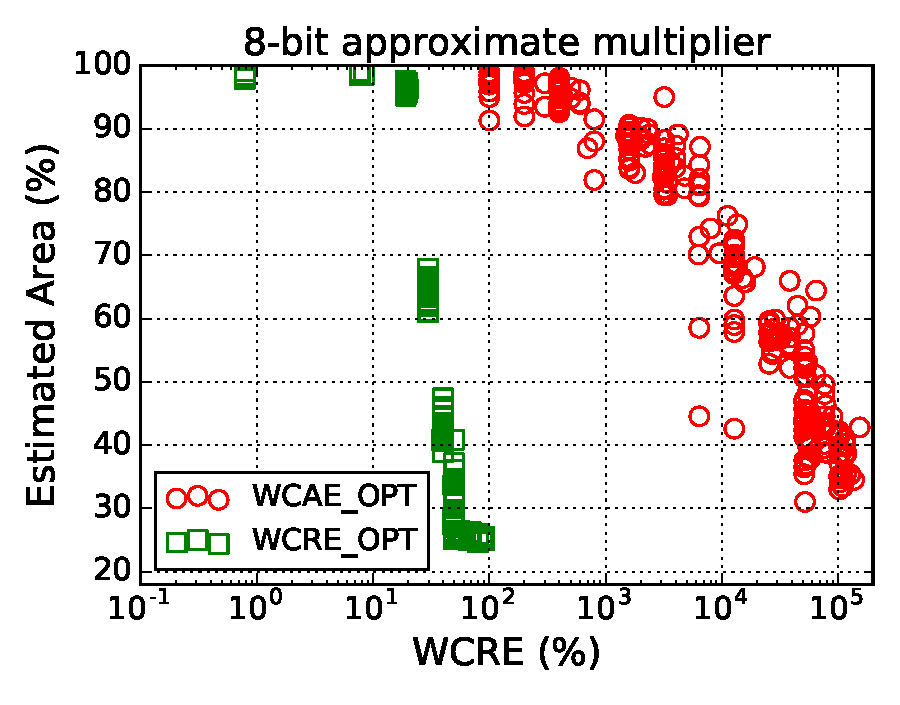
\includegraphics[width=0.42\textwidth]{img/multApprox8_WCRE.pdf}
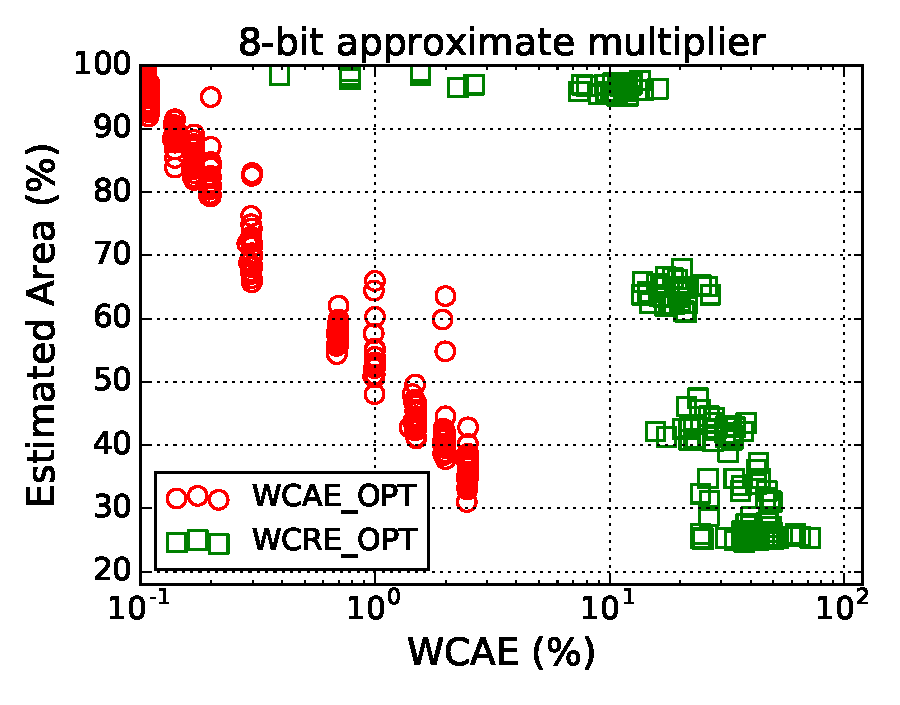
\includegraphics[width=0.42\textwidth]{img/multApprox8_WCAE.pdf}
\vspace{-1.5em}
\caption{A comparison of 8-bit multipliers approximated for WCRE and WCAE.} 
\label{mult_pareto_wre}
\label{fig:comp}
%\vspace{-1em}
\end{figure}

% ----------------------------------------------------------------
%\subsection{Evaluating the Error of Approximate Circuits}
% ----------------------------------------------------------------
\vspace{0.5em}

\emph{Methods evaluating the approximation error} have a crucial impact on the
performance of the approximation process. A popular class of methods employs
\emph{circuit simulation}  on a set of inputs to evaluate the error. Such
methods typically suffer from low scalability (when an exhaustive simulation is
applied) or a lack of guarantees (when the circuits are simulated for a subset
of the possible inputs only). In order to provide guarantees on the
approximation error and scale to complex circuits at the same time, various
\emph{formal verification} techniques, such as model-checking, SAT solving, or
BDDs have recently been integrated to the approximation
process~\cite{Ciesielski15,Vasicek:DATE17}. They typically employ auxiliary
circuits, so-called \emph{miters}, that combine the original circuit and the
approximate circuit and evaluate the error~\cite{drechsler-DAC'16}. In our
previous work~\cite{iccad17}, we proposed a~miter construction allowing one to
subsequently use an efficient SAT-based procedure to check whether the
approximate circuit satisfies a given WCAE bound. Moreover, we proposed a
verifiability-driven search-strategy that drives the search towards promptly
verifiable approximate circuits. The strategy introduces a limit on resources
that the underlying SAT solver can use to prove that the WCAE bound is met.
This approach currently provides the best performance for the circuit
approximation with WCAE guarantees.



% ================================================================
\section{SAT-based WCRE Evaluation}
% ================================================================

To evaluate whether the given approximate circuit meets the required bound on
WCRE, we adapt and extend the miter we designed for WCAE~\cite{iccad17}. As
shown in Figure~\ref{fig:miter_wcae} (left), the miter interconnects the golden
circuit $G$ and the candidate circuit $C$ that both share identical inputs. The
subtractor and absolute value blocks allow us to quantify the approximation
error between $C$ and $G$. Finally, the error is compared to a given threshold
value $T$, and the output of the comparator is set to logical $true$ if and only
if the threshold $T$ is violated. Thus the miter construction allows us to
evaluate whether $WCAE(C,G) > T$ in a single SAT query. Note that, for a given
approximation scenario, the threshold $T$ is constant and can therefore be built
into the structure of the comparator.

\begin{figure}[t]
    \centering
    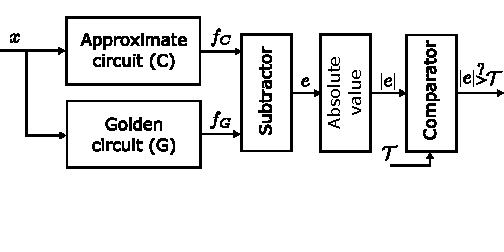
\includegraphics[width=0.45\textwidth]{img/excel/miter_wcae.pdf}
    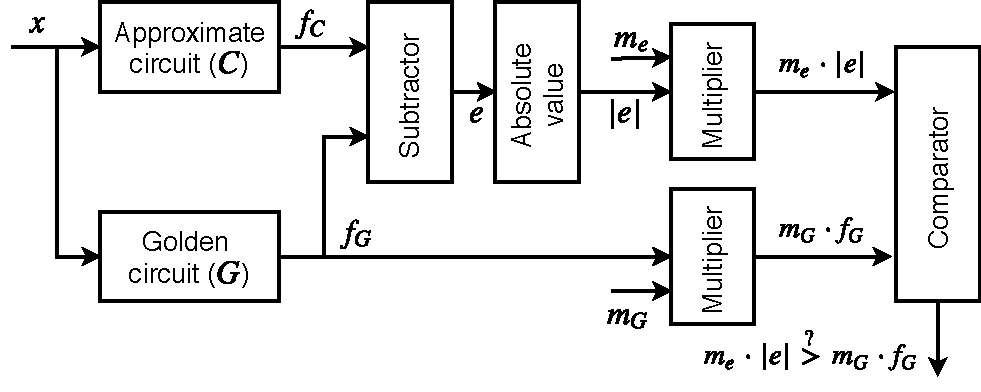
\includegraphics[width=0.53\linewidth]{img/excel/miter_wcre.pdf}
    \vspace{-1em}
    \caption{The approximation miter used for WCAE evaluation (left) and 
    the novel construction for WCRE evaluation (right).}
    \label{fig:miter_wcae}
    \vspace{-1em}
\end{figure}
 
% ----------------------------------------------------------------
\subsection{A Generic WCRE Miter}
% ----------------------------------------------------------------

To obtain a WCRE miter, we extend the WCAE miter by adding some components.
Recall that we need to check the satisfiability  of the following formula:
%
\begin{equation} \label{eq:maxT} \max_{n \in \mathbb{N}} \frac{\left|f_{G}(n) -
f_{C}(n)\right|}{f_{G}(n)} > T.  \end{equation} 

Note that we do not need to find the maximum of the left-hand side of the
formula, but rather determine if there exists a single input combination for
which the bound $T$ is violated. Therefore, we can replace
Formula~\ref{eq:maxT} by the following constraint
%
\begin{equation} \label{eq:wcre_final} \exists n \in N: \left|f_{G}(n) -
f_{C}(n)\right| * m_{e} > f_{G}(n) * m_{G} \end{equation}
%
where $T = m_{G} / m_{e}$. Based on this formula, we build a general WCRE miter
using  two multipliers by a constant and a generic comparator, see
Figure~\ref{fig:miter_wcae} (right).


%By an analysis of Formula~\label{er:wcre_final} we can identify the components
%needed to construct the approximation miter. In addition to the elements of the
%original WCAE miter, we also have to utilise two multipliers by constant and a
%generic comparator. The resulting miter construction is illustrated in
%Figure~\ref{fig:miter_wcre} and allows us to decide, whether a candidate
%solution violates an arbitraty threshold on the WCRE metric using a single SAT
%query.

%\begin{figure}[t]
%    \centering
%    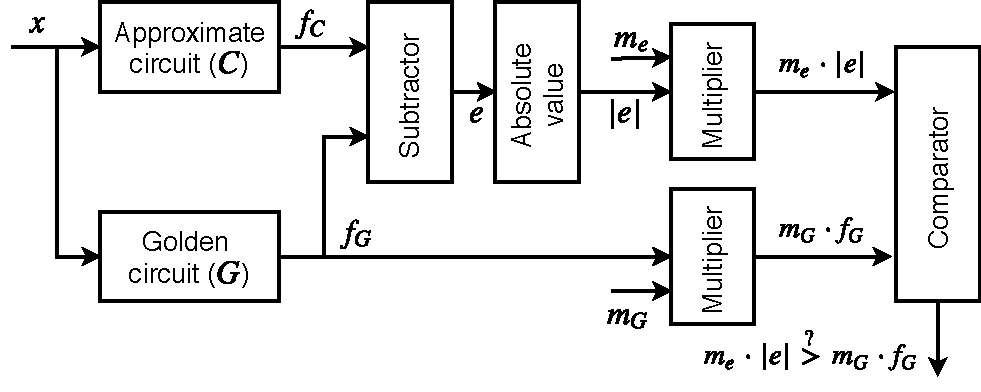
\includegraphics[width=0.8\linewidth]{img/excel/miter_wcre.pdf}
%    \vspace{-1em}
%    \caption{New approximation miter used for general WCRE evaluation.}
%    \label{fig:miter_wcre}
%\end{figure}


% ----------------------------------------------------------------
\subsection{Variants of the WCRE Miter}    
% ----------------------------------------------------------------

Observe that the resulting WCRE miter is larger and more complex than the WCAE
miter. This indeed slows down its evaluation and thus reduces the overall
performance of the approximation process. To improve the performance and
scalability  with respect to the circuit complexity, we simplify the general
WCRE miter and propose three variants of the miter that are smaller but can be
used for certain values of the bound $T$ only.

As we work with the binary representation of integers, multiplication by the
powers of 2 is identical to a bit shift operation. Thus, each of the constants
$m_{G}$ and $m_{e}$ can be expressed using two values: namely, $mc_{x}$ denoting
a multiplicative constant and $bs_{x}$ denoting a number of shifted bits. The
original values of $m_{G}$ and $m_{e}$ are then computed as:

\vspace{-12mm}
\begin{multicols}{2}
$$m_{G} = mc_{G} * 2^{bs_{G}}$$
\break
$$m_{e} = mc_{e} * 2^{bs_{e}}$$
\end{multicols}
\vspace{0mm}

In combinational circuits, a shift by a constant number of bits is represented
by a~reconnection of wires only and does not contain any logical gates. This
setting allows us to remove one or even both of the constant multiplications for
a subset of target WCRE error bounds $T$. 
%
If we restrict the values of $m_g$ and $m_e$ to powers of two, we suffice with
utilising bit shifts only. This restricts the obtainable values of $T$ to
$1/2^{bs_{e}}$, e.g., $50\ \%$, $25\ \%$, or $12.5\ \%$. Adding one multiplier
by a constant significantly broadens the range of supported target values. These
can be expressed by one of the formulas: $2^{bs_{G}} / (mc_{e} * 2^{bs_{e}})$ or
$(mc_{G} * 2^{bs_{G}}) / 2^{bs_{e}}$. However, the constants should be kept
small. Using higher values leads to larger bit widths representing the compared
numbers, and therefore a more complex comparator, thus negating the contribution
of this optimisation.

%A detailed comparison of the proposed miter architectures is presented in the
%experimental evaluation.

%The generic WCRE miter, shown in Figure~\ref{fig:miter_wcre}, consists of the
%inspected approximate circuit $C$, the golden circuit $G$ which serves as
%specification, a subtractor and a~comparator which checks whether the
%\emph{absolute error} caused by approximation is greater than a given threshold
%$T$. The output of the miter is a single bit which evaluates to 1 if the error
%is violated as shown below: \[ |e| > T \]
%
%\noindent Where $|e|$ is \emph{absolute error}: \[\left| e \right| = \left|
%\text{uint}(f_C(x)) - \text{uint}(f_G(x)) \right| \]
%
%\noindent $\text{uint}(x)$ denotes the unsigned integer representation of a bit
%vector $x$. 
%

%%\begin{figure}[t]
%%    \centering
%%    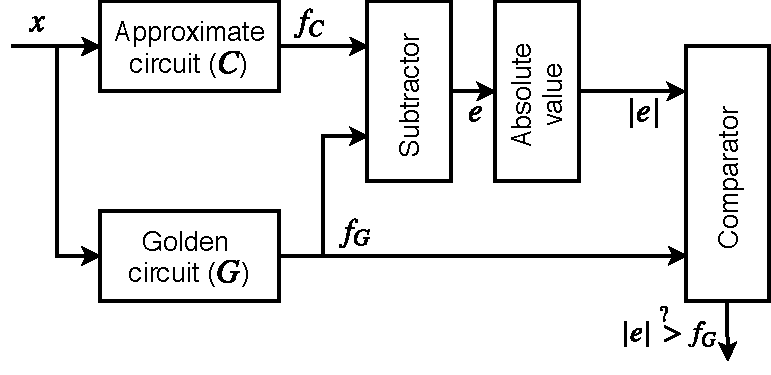
\includegraphics[scale=0.5]{img/miter_100.pdf}
%%    \caption{Approximation miter used for 100\% WCRE}
%%    \label{fig:miter_100}
%%\end{figure}

%% ----------------------------------------------------------------
%\subsection{100\% WCRE Miter}    
%% ----------------------------------------------------------------

%By a simple adjustment we can derive 100\% WCRE miter from the WCAE miter as
%shown in Figure~\ref{fig:miter_100}. Essential parts of miter -- approximate
%circuit $C$, golden circuit $G$ and subtractor, stay the same as in WCAE miter.
%However, the comparator needs to be changed from a comparator of absolute error
%$|e|$ with a constant $T$ to a comparator of absolute error $|e|$ with output
%from the golden circuit $f_G$. The inequation given by this miter is shown
%below: \[ \left| e \right| > \text{uint}(f_G(x)) \]
%
%\noindent If \( \text{uint}(f_G(x)) \not= 0 \) then we can transform the
%previous inequation into following: \[ \frac{\left| e
%\right|}{\text{uint}(f_G(x))} > 1 \]    
%
%\noindent Left side of inequation calculates \emph{relative error} for an~input
%vector $x$. If this \emph{relative error} is for any input vector $x$ greater
%than 1, the 100\%~WCRE is violated. As for the miter, its output is again a
%single bit which evaluates to 1 if the WCRE is violated.
%
%100\% WCRE miter, however, is not very useful because even a circuit which for
%every input vector $x$ returns $\text{uint}(f_C(x)) =~0$ satisfies the 100\%
%WCRE. That is certainly not a behaviour expected from an~approximate circuit.

%% ----------------------------------------------------------------
%\subsection{General WCRE Miter} %
%----------------------------------------------------------------
%
%To create a miter able to calculate whether any set WCRE is violated we need to
%add two constant multipliers to the 100\% WCRE miter, one to the output of the
%golden circuit $f_G$ and other to the output of the absolute value block~$|e|$.
%Their outputs are then connected to the comparator as shown in
%Figure~\ref{fig:miter_wcre}. By managing the values of constant inputs of
%multipliers i.e. $m_{|e|}$ and $m_G$, where \( m_{|e|}, m_G \in \mathbb{N} \),
%we can evaluate arbitrary WCRE. The inequation given by this miter is shown
%below: \[ \left| e \right| \cdot m_{|e|} > \text{uint}(f_G(x)) \cdot m_G \]
%
%\noindent If \( \text{uint}(f_G(x)) \not= 0 \) and \( m_{|e|}, m_G \in
%\mathbb{N} \) then we can transform the previous inequation into following: \[
%\frac{\left| e \right|}{ \text{uint}(f_G(x)) } > \frac{m_G}{m_{|e|}} \]
%
%\noindent From this inequation it is clear that by setting $m_G$ and $m_{|e|}$
%we are able to obtain any WCRE and subsequently check whether this WCRE is
%violated for some input vector $x$. 
%
%
%% ----------------------------------------------------------------
%\subsection{Implementation of WCRE Miter} %
%---------------------------------------------------------------- 
% 
%In order to implement the general WCRE miter we needed to make some changes to
%the absolute value subtractor and we also added a possibility to bit-shift the
%inputs of constant multipliers. By bit-shifting we are able to multiply or
%divide the output of either golden circuit $f_G$ or absolute value subtractor
%$|e|$ by the powers of 2 and create miters with 50\%, 25\%, 12,5\%, 6,25\%,...
%WCRE.
%
%The use of bit-shifts allows us to reduce the complexity of the miter and
%therefore achieve faster evaluation of miter. Because the evaluation of miters
%is the most critical and time consuming part of CGP loop, it is of great
%importance. Comparison of evaluation speeds of miters of 4 to 32 bit adders in
%the task of adder approximation can be seen in Figure~\ref{fig:evals}
%(evaluations per second are shown in logarithmic scale). Miters using only
%bit-shifts (cyan) have clearly the fastest evaluation speed, but are closely
%followed by miters with a single multiplier (green) and miters with two
%multipliers (red). It is worth noting that simulation of circuits (blue) is
%better for circuits with small bit-width but for circuits with bit-width
%greater than 10 bits it can no longer effectively solve the problem.

%\begin{figure}[t]
%    \centering
%    \includegraphics[scale=0.32]{img/addApprox_log.pdf}
%    \caption{Comparison of evaluation speed of different WCRE miters and 
%     simulation}
%    \label{fig:evals}
%\end{figure}

%In this paper, we propose a novel approach for designing approximate arithmetic
%circuits with formal guarantees on the \emph{worst-case relative error} (WCRE).
%For an original circuit $C$ computing a function $f_{C}$ and its approximation
%$C'$  computing a function $f_{C'}$,$\mbox{WCRE}(C,C')  = \max_{n \in
%\mathbb{N}} \frac{\left|f_{C}(n) - f_{C'}(n)\right|}{max(1, f_{C}(n))}$. Such
%circuits play an important role in many application domains including, e.g.,
%approximation of HW-accelerated architectures for neural
%networks~\cite{Judd:2016} and other soft-computing applications~\cite{sfc}. 

% ================================================================
\section{Experimental Evaluation}
% ================================================================

We have integrated the proposed WCRE miters into our tool ADAC~\cite{ADAC} and
evaluated its performance on a benchmark of  circuit approximation problems.

% ----------------------------------------------------------------
\subsection{Comparison of the WCRE Miters}
% ----------------------------------------------------------------
%
In Table~\ref{tab:miter-params},  we compare the size of the proposed WCRE
miters. We select three target WCRE bounds $T$ for the bit-shift variant and
four target error values for one and two multiplier miter designs. The table
shows the average sizes of the different variants of the miter obtained for the
three chosen bit widths in adder and multiplier approximation. The size is
measured in the number of nodes in the AIG graph representation of the miter.
Note that AIG is a basic representation of circuits in ADAC and is directly used
as the input for the SAT solving procedure. A larger size of AIGs negatively
affects the performance of the solver. We can see that the bit-shift variant is
about a~factor 2 smaller than the general construction using two multipliers.
For multipliers, the differences in the size between the variants are less
significant as the circuits themselves form  a bigger part of the miter. Note
that the average size of the WCAE miter for a 32-bit adder and 12-bit multiplier
is 810 and 2437 AIG nodes, respectively, which is smaller than even the
bit-shift variant of the WCRE miters for the corresponding circuits. This
clearly indicates that the evaluation against WCRE is considerably harder.

\begin{table}[t]

\centering
\renewcommand{\arraystretch}{1.08}
\caption{Numbers of AIG nodes for different miters and WCAE bounds $T$.}
\label{tab:miter-params}
\begin{tabular*}{\textwidth}{@{\extracolsep{\fill}}l|rrr|rrrr|rrrr}
\multicolumn{1}{c|}{} & \multicolumn{3}{c|}{\textbf{Bit shifts}} & \multicolumn{4}{c|}{\textbf{One multiplier}} & \multicolumn{4}{c}{\textbf{Two multipliers}} \\ \hline
\multicolumn{1}{c|}{\textbf{T} [\%]} & \multicolumn{1}{c}{\textbf{12.5}} & \multicolumn{1}{c}{\textbf{25.0}} & \multicolumn{1}{c|}{\textbf{50.0}} & \multicolumn{1}{c}{\textbf{10.0}} & \multicolumn{1}{c}{\textbf{33.3}} & \multicolumn{1}{c}{\textbf{66.7}} & \multicolumn{1}{c|}{\textbf{80.0}} & \multicolumn{1}{c}{\textbf{30.0}} & \multicolumn{1}{c}{\textbf{42.9}} & \multicolumn{1}{c}{\textbf{71.4}} & \multicolumn{1}{c}{\textbf{85.7}} \\ \hline
\textbf{add8} & 226 & 228 & 233 & 324 & 327 & 342 & 360 & 447 & 510 & 506 & 519 \\
\textbf{add16} & 497 & 501 & 502 & 770 & 755 & 773 & 756 & 1079 & 1225 & 1181 & 1220 \\
\textbf{add32} & 1120 & 1090 & 1114 & 2074 & 2116 & 2084 & 2106 & 3125 & 3249 & 3315 & 3354 \\ \hline
\textbf{mult4} & 268 & 267 & 273 & 335 & 347 & 356 & 347 & 464 & 499 & 492 & 513 \\
\textbf{mult8} & 1175 & 1177 & 1183 & 1393 & 1421 & 1436 & 1414 & 1685 & 1833 & 1803 & 1841 \\
\textbf{mult12} & 2617 & 2621 & 2622 & 3032 & 3057 & 3060 & 3051 & 3512 & 3748 & 3726 & 3756
\end{tabular*}
%\vspace{-1em}
\end{table}


\begin{figure}[t]
    \centering
    \includegraphics[width=0.49\textwidth]{img/prezentace/addApprox_log.pdf}
    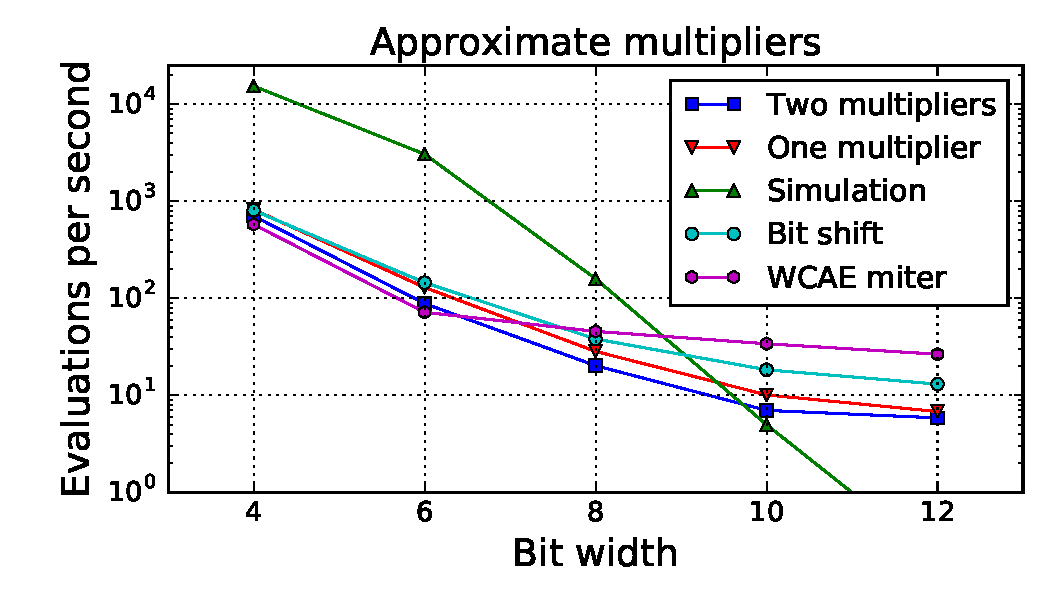
\includegraphics[width=0.49\textwidth]{img/prezentace/multApprox_log.pdf}
    \vspace{-1em}
    \caption{Performance of  the circuit evaluation using different WCRE miters,
    the WCAE~miter, and simulation. Left: Adders. Right: Multipliers.}  
    \label{fig:evals}
    \vspace{-1em}
\end{figure}

Figure~\ref{fig:evals} illustrates how the size of the miters affects the
performance of the candidate circuit evaluation. In particular, it shows the
average number of evaluations per second (taken from 20 independent runs) when
the approximation of adders (left) and multipliers (right) with different
bit-widths (the  $x$-axis) is performed. We also compare the miter-based methods
with full simulation and WCAE miter evaluation.

We can observe that the simulation is considerably faster for small bit-widths,
however, its performance  significantly drops for circuits with operands larger
than 10-bits. The proposed-SAT based approach scales much better. For the
adders, it provides very good performance (around 100 evaluations per second)
even for 32-bit operands. For the multipliers (representing structurally more
complex circuits), the performance is much lower and drops to 10 evaluations per
second for 12-bit operands. As expected, the speed of the miter evaluation slows
down with increasing miter complexity---the bit-shift variant is the fastest
while the version with two multipliers is the slowest. The difference in the
evaluation speed is negligible for smaller circuits but becomes more significant
for larger bit-widths. Note that the evaluation of the WCAE miters is
significantly faster due their smaller sizes (e.g. 4-times smaller for the
32-bit adders and 1.5-times smaller for the 12-bit multipliers in comparison to
the two multiplier implementation).

For larger miters, the bounds on the SAT solver resources get applied, and a
small number of circuit evaluation tasks is skipped (e.g., for the WCRE mitters,
$0.7\ \%$ for the 32-bit adders and $6\ \%$ for the 12-bit multipliers). The
idea is to skip candidates for which the evaluation takes too long because their
successors typically have the same problem and thus they reduce the performance
of the overall approximation process. For more details, see our previous
work~\cite{iccad17}, where we introduced this, so-called verifiability-driven
strategy.

\begin{figure}[t]
    \centering
    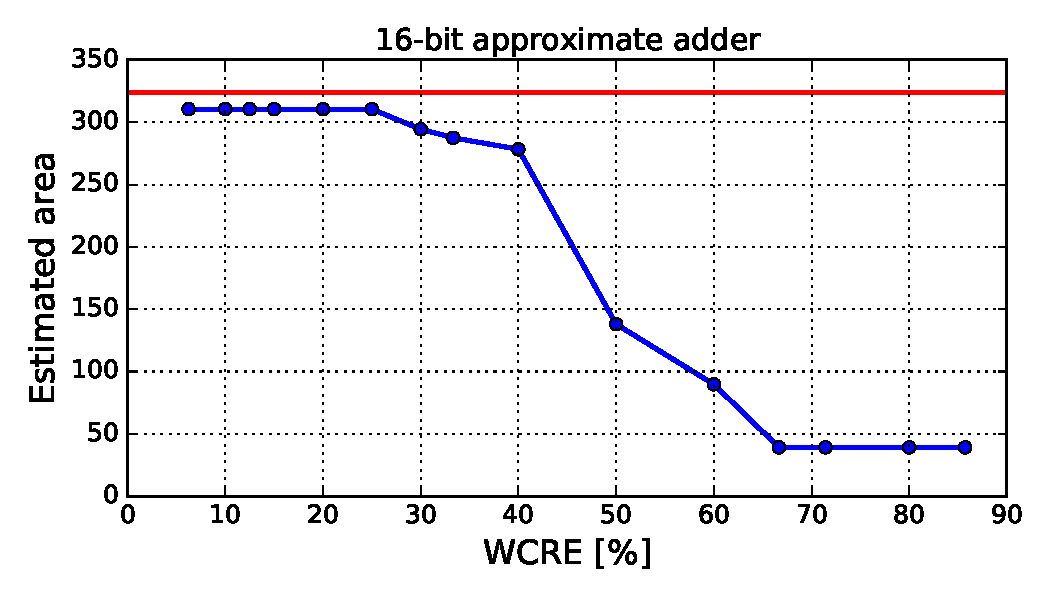
\includegraphics[width=0.49\textwidth]{img/prezentace/medians-addApprox16-area.pdf}
        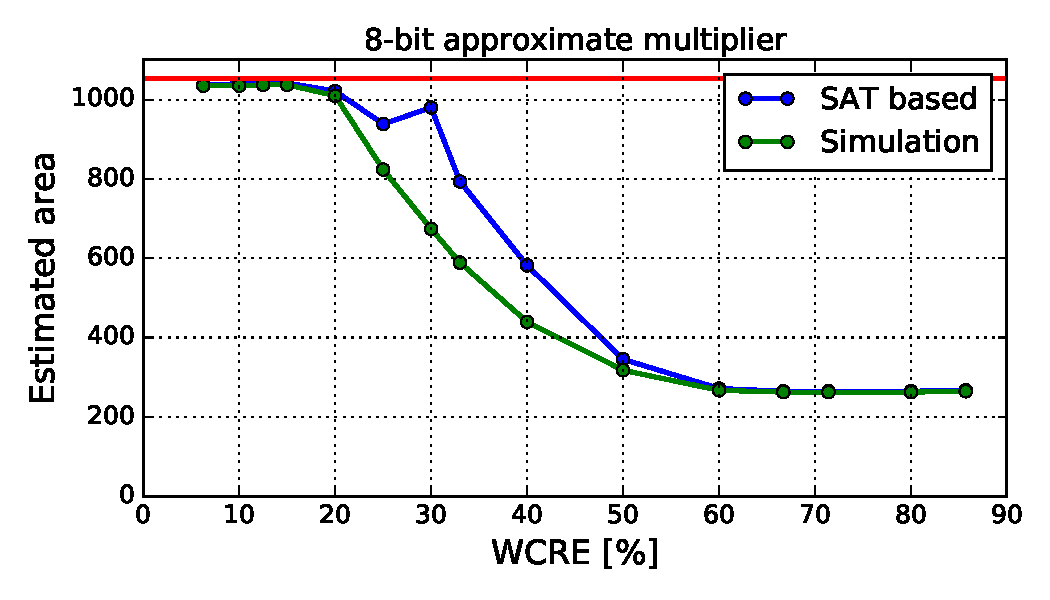
\includegraphics[width=0.49\textwidth]{img/prezentace/medians-multApprox8-area.pdf}
        \vspace{-0.9em}
    \caption{The median circuit area of approximate adders (left) and multipliers 
    (right). The red line indicates the area of the original circuit.}
    \label{fig:adders}
    \vspace{-1em}
\end{figure}

% ----------------------------------------------------------------
\subsection{Circuit Approximation}
% ----------------------------------------------------------------

In this section, we study how the proposed SAT-based circuit evaluation can be
leveraged in circuit approximation. Recall that we integrate the evaluation
procedure into the verifiability-driven circuit approximation based on Cartesian
genetic programming. The optimisation is formulated as a single-objective
optimisation, i.e., for a given threshold on the WCRE bound~$T$, the
approximation seeks for a circuit satisfying the bound and having the smallest
circuit area\footnote{We estimate the area as the sum of sizes of the gates (in
the target 45~nm technology) used in the circuit. The estimation tends to be
accurate and also adequately captures the circuit power
consumption~\cite{Vasicek:DATE17}.}. For every value of $T$, we run a
2-hours-long approximation process. To take into account the randomness of the
evolutionary optimisation, we report the median of the circuit area obtained
from 20 independent runs. Figure~\ref{fig:adders} illustrates the results of the
approximation process, in particular, the obtained approximate circuits for the
16-bit adders (left) and the 8-bit multipliers (right). The circuits form a
Pareto front that captures the trade-offs between the area and the approximation
error. The red line shows the area of the golden circuit. 

For the \emph{adders}, the proposed approximation method works very well and is
able to successfully approximate circuits up to 32-bit operands (not presented
here). Figure~\ref{fig:adders} (left) shows that, for 16-bit adders, the most
interesting solutions in the terms of accuracy and area savings are located in
the interval between $30\ \%$ and $60\ \%$ WCRE. For smaller target error
values, the reduction of the circuit size is negligible. On the other hand, the
solutions with larger approximation errors do not feature further improvements.
We can also observe  a dramatic area reduction between $40\ \%$ and $50\ \%$
WCRE.

% ----------------------------------------------------------------
%\subsection{Approximate Multipliers}
% ----------------------------------------------------------------

Approximation of the \emph{multipliers} represents a significantly harder
problem. Recall that the size of multipliers (and thus also of the miters) grows
quadratically with respect to their bit-widths. Therefore, the design space is
larger and candidate evaluation is more complicated as discussed in the previous
section. Figure~\ref{fig:adders} (right) compares the approximate 8-bits
multipliers obtained using the simulation-based and SAT-based evaluation
procedure. The SAT-based approach slightly lags behind the simulation mainly in
the interval between $25\ \%$ and $40\ \%$ WCRE. This can be explained by the
worse  performance of the SAT-based evaluation on the 8-bit multipliers (recall
Figure~\ref{fig:evals} (right)).  

As the performance of the simulation-based evaluation is very low beyond 10-bit
multipliers, the approximation process is not able to provide a good
approximation of these circuits within a 2-hours-long run. Although the
SAT-based approach (namely the bit-shift solution) is able to evaluate around
10~candidates per second (for the 12-bit multipliers), the approximation process
also fails to provide good Pareto sets. This is probably caused by the
candidates that are skipped during the evaluation due to the resource limits on
the underlying SAT solver. Note that this behaviour was not observed for the
WCAE approximation that works very well even for 16-bit multipliers despite many
skipped solutions~\cite{iccad17}. This again indicates that the WCRE
approximation is very challenging, and future research is necessary in this
area.

% to achieve practically useful~results.

%\begin{figure}[t]
%    \centering
%
%    \caption{Median circuit area of approximate multipliers designed using SAT based approach and simulation.}
%    \label{fig:mults}
%\end{figure}




%% ================================================================
%\section{Conclusion}
%% ================================================================
%TODO In our work, we focus on designing approximate circuits that provide good area savings while featuring
%acceptable worst-case absolute and worst-case relative error. In particular, we designed novel miter construction evaluating WCRE and integrated it into our
%framework [?] that has been focused purely on WCAE.
%Presented miter design provides best performance for
%adders (up to 32 bits) but for now lacks behind in
%other more complex arithmetic circuits. Our future
%aspirations are to improve the miter construction to
%scale better with more complex circuits and allow the
%optimisation of other arithmetic circuits.
%
%




%\section*{Extended Abstract}

%, and
%the multi\-ply-accumulate-transform structures of artificial neurons in neural
%networks (consuming about 50\% of the total power in neural network
%accelerators~\cite{Judd:2016}). 


%We build on our evolutionary-driven approximation techniques~\cite{iccad17} ensuring the worst-case absolute error (WCAE). We first demonstrate that ensuring bounds on the relative error is a more challenging problem:  (1)  bounds on the relative error typically enable smaller reductions in the circuit logic since the part of the circuit responsible for small output values has to be at least partially preserved and (2) evaluating the relative error is computationally more demanding. To mitigate the latter issue and to achieve scalability for complex circuits going beyond 16-bit multipliers, we introduce a~new construction of the so-called miters, i.e., circuits that compose outputs of the original and approximated circuits, uniting these two circuits into a single one, on which checking of the WCRE bounds can be performed~\cite{miter}. This allows us to effectively utilize powerful SAT solving techniques for circuit evaluation. We then explore and compare the structure of approximate circuits optimised for the absolute and relative error, and various also their functional and non-functional circuit parameters.


%\textcolor{red}{How we can demonstrate that WCRE offers less space for reduction comparing to WCAE -- comparing the error expressed in percents does not make much sense.}
%In our work, we also focus on designing new circuits that provide good area savings while featuring acceptable WCAE and WCRE. In particular, we integrate the WCRE evaluation into our framework~\cite{ADAC} that has been focused purely on WCAE.


%\vspace{2em}
%\noindent
%\textcolor{red}{[Create a figure demonstrating that the relative error is a more challenging problem as it enables smaller reductions  in the circuit logic. Also show that circuits optimising the relative error typically lead to a pure absolute errors and vice versa.]}
%
%
%\vspace{2em}
%\noindent


% ---- Bibliography ----
%
% BibTeX users should specify bibliography style 'splncs04'.
% References will then be sorted and formatted in the correct style.
%
\bibliographystyle{splncs04}
\bibliography{mybibliography}
%



\end{document}
